% DPF 09 talk on strangeness in nucleon

\documentclass[10pt]{beamer}
\usepackage{amsmath}
\usepackage{mathtools}
\usefonttheme{professionalfonts}
\usefonttheme{serif}
%\documentclass[12pt]{beamerthemeSam.sty}
\usepackage{epsf}
%\usepackage{pstricks}
%\usepackage[orientation=portrait,size=A4]{beamerposter}
\geometry{paperwidth=160mm,paperheight=120mm}
%DT favorite definitions
\def\LL{\left\langle}	% left angle bracket
\def\RR{\right\rangle}	% right angle bracket
\def\LP{\left(}		% left parenthesis
\def\RP{\right)}	% right parenthesis
\def\LB{\left\{}	% left curly bracket
\def\RB{\right\}}	% right curly bracket
\def\PAR#1#2{ {{\partial #1}\over{\partial #2}} }
\def\PARTWO#1#2{ {{\partial^2 #1}\over{\partial #2}^2} }
\def\PARTWOMIX#1#2#3{ {{\partial^2 #1}\over{\partial #2 \partial #3}} }

\def\rightpartial{{\overrightarrow\partial}}
\def\leftpartial{{\overleftarrow\partial}}
\def\diffpartial{\buildrel\leftrightarrow\over\partial}

\def\BI{\begin{itemize}}
\def\EI{\end{itemize}}
\def\BE{\begin{displaymath}}
\def\EE{\end{displaymath}}
\def\BEA{\begin{eqnarray*}}
\def\EEA{\end{eqnarray*}}
\def\BNEA{\begin{eqnarray}}
\def\ENEA{\end{eqnarray}}
\def\EL{\nonumber\\}


\newcommand{\map}[1]{\frame{\frametitle{\textbf{Course map}}
\centerline{\includegraphics[height=0.86\paperheight]{../../map/#1.png}}}}
\newcommand{\wmap}[1]{\frame{\frametitle{\textbf{Course map}}
\centerline{\includegraphics[width=0.96\paperwidth]{../../map/#1.png}}}}

\newcommand{\etal}{{\it et al.}}
\newcommand{\gbeta}{6/g^2}
\newcommand{\la}[1]{\label{#1}}
\newcommand{\ie}{{\em i.e.\ }}
\newcommand{\eg}{{\em e.\,g.\ }}
\newcommand{\cf}{cf.\ }
\newcommand{\etc}{etc.\ }
\newcommand{\atantwo}{{\rm atan2}}
\newcommand{\Tr}{{\rm Tr}}
\newcommand{\dt}{\Delta t}
\newcommand{\op}{{\cal O}}
\newcommand{\msbar}{{\overline{\rm MS}}}
\def\chpt{\raise0.4ex\hbox{$\chi$}PT}
\def\schpt{S\raise0.4ex\hbox{$\chi$}PT}
\def\MeV{{\rm Me\!V}}
\def\GeV{{\rm Ge\!V}}

%AB: my color definitions
%\definecolor{mygarnet}{rgb}{0.445,0.184,0.215}
%\definecolor{mygold}{rgb}{0.848,0.848,0.098}
%\definecolor{myg2g}{rgb}{0.647,0.316,0.157}
\definecolor{abtitlecolor}{rgb}{0.0,0.255,0.494}
\definecolor{absecondarycolor}{rgb}{0.0,0.416,0.804}
\definecolor{abprimarycolor}{rgb}{1.0,0.686,0.0}
\definecolor{Red}           {cmyk}{0,1,1,0}
\definecolor{Grey}           {cmyk}{.7,.7,.7,0}
\definecolor{Lg}           {cmyk}{.4,.4,.4,0}
\definecolor{Blue}          {cmyk}{1,1,0,0}
\definecolor{Green}         {cmyk}{1,0,1,0}
\definecolor{Brown}         {cmyk}{0,0.81,1,0.60}
\definecolor{Black}         {cmyk}{0,0,0,1}

\usetheme{Madrid}


%AB: redefinition of beamer colors
%\setbeamercolor{palette tertiary}{fg=white,bg=mygarnet}
%\setbeamercolor{palette secondary}{fg=white,bg=myg2g}
%\setbeamercolor{palette primary}{fg=black,bg=mygold}
\setbeamercolor{title}{fg=abtitlecolor}
\setbeamercolor{frametitle}{fg=abtitlecolor}
\setbeamercolor{palette tertiary}{fg=white,bg=abtitlecolor}
\setbeamercolor{palette secondary}{fg=white,bg=absecondarycolor}
\setbeamercolor{palette primary}{fg=black,bg=abprimarycolor}
\setbeamercolor{structure}{fg=abtitlecolor}

\setbeamerfont{section in toc}{series=\bfseries}

%AB: remove navigation icons
\beamertemplatenavigationsymbolsempty
\title[Work and potential energy]{
  \textbf {Work and potential energy}\\
%\centerline{}
%\centering
%\vspace{-0.0in}
%\includegraphics[width=0.3\textwidth]{propvalues_0093.pdf}
%\vspace{-0.3in}\\
%\label{intrograph}
}

\author[W. Freeman] {Physics 211\\Syracuse University, Physics 211 Spring 2022\\Walter Freeman}

\date{\today}

\begin{document}

\frame{\titlepage}


\frame{\frametitle{\textbf{Tuesday's class}}
	\large
	
\BI
\item Many of you told me that you appreciated the format on Tuesday where you did an exercise in class.
\item ... so we can do this again in the future!

\vspace{.5in}

\item However:
\BI
\item That exercise took longer in class than I had anticipated
\item We didn't get as far into the {\it application} of the work-energy theorem as I had hoped
\item I didn't have a chance to revise the recitation material on Wednesday
\item ... so we are pushing the schedule back by about half a class. (This is fine!)
\item We have some flexibility at the end of the semester and everything will work out
\EI
\EI
}




\frame{\frametitle{\textbf{Announcements}}
\BI
\item{Your next homework assignment is due next Wednesday.}
\item Please come prepared to ask questions next Tuesday
\EI 
}
%
%\frame{\frametitle{\textbf{Exam 2 recap}}
%\centerline{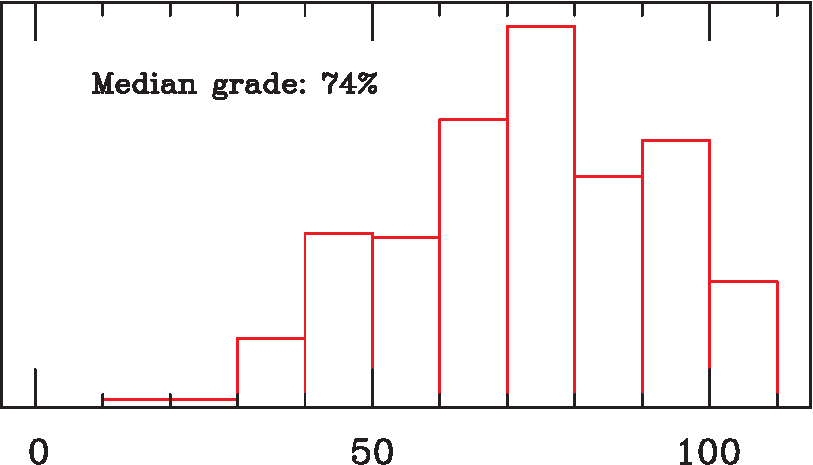
\includegraphics[width=0.5\textwidth]{exam2histo-crop.pdf}}
%    \Large
%    \centerline{This exam was quite difficult and most of you did very well!}
%\BI
%\item 64 F's \pause
%\item 16 D's \pause
%\item 69 C's \pause
%\item 121 B's \pause
%\item \color{Red} 154 (!) A's \pause
%\EI
%
%\pause
%
%\large
%\centerline{There was no evidence that either alternate exam was harder than Thursday's.}
%
%}

\frame{\frametitle{\textbf{Where we've been and where we're going}}
  \BI
  \large
\item{Last time: kinetic energy and the work-energy theorem}
\item{This time: the idea of potential energy and conservation of energy}
\BI
\item{Potential energy: ``the most meaningful bookkeeping trick in physics''}
\item{Lets us understand many phenomena without difficult mathematics}
\item{Conservation of energy: there's always the same amount of energy, and it just changes forms}
\EI
\EI
}

\frame{\frametitle{\textbf{Review: kinetic energy}}
\large
We will see that things are often simpler when we look at something called ``energy''
\BI
\item{Basic idea: don't treat $\vec a$ and $\vec v$ as the most interesting things any more}
\item{Treat $v^2$ as fundamental: $\frac{1}{2}mv^2$ called ``kinetic energy''}
  \EI
  \bigskip
  \begin{columns}
    \column{0.5\textwidth}
    \color{Blue}
    \centerline{Previous methods:}
    \BI
    \color{Blue}
  \item{Velocity is fundamental}
  \item{Force: causes velocities to change over time}
  \item{Intimately concerned with vector quantities}
  \EI
    \column{0.5\textwidth}
    \color{Red}
    \centerline{Energy methods:}
    \BI
    \color{Red}
  \item{$v^2$ (related to kinetic energy) is fundamental}
  \item{Force: causes KE to change over distance}
  \item{Energy is a {\it scalar}}
    \EI
  \end{columns}
  
  \bigskip
  \bigskip
  
  \centerline{Energy methods: useful when you don't know and don't care about time}
}

\frame{\frametitle{\textbf{Energy: measurements and units}}
\large
We didn't talk about how we {\it measure} energy last time:

\bigskip

\centerline{Kinetic energy = $\frac{1}{2}mv^2$}
\BI
\item{Energy has units $\rm kg\, m^2/s^2$}
\item{This unit is called a {\it joule}}
\item{1 joule = the energy required to lift an apple one meter}
\item{This is also the unit for work}
\EI
%
%\centerline{A new idea: power, the rate of doing work}
%
%\BI
%\item Sometimes we are interested in the rate at which a force does work
%\item This idea is called {\it power}, and it is measured in joules per second
%\item A joule per second is also called a watt
%\item If $W = \vec F \cdot \Delta \vec s$, then I can take derivatives of both sides to get...
%\item $P = \vec F \cdot \vec v$
%\item You'll need this in recitation tomorrow
%\EI

}

\frame{\frametitle{\textbf{The work-energy theorem in 1D}}
Last time we saw the ``work-energy theorem'' was a consequence of simple kinematics:
\begin{equation*}
  \frac{1}{2} mv_f^2 - \frac{1}{2} mv_0^2 = F \Delta x
\end{equation*}

\bigskip
\bigskip
\bigskip
\pause

Or in more than one dimension:
\begin{equation*}
  \frac{1}{2} mv_f^2 - \frac{1}{2} mv_0^2 = \vec F \cdot \Delta \vec s = (F_\parallel)(\Delta s) = (F)(\Delta s_\parallel)
\end{equation*}


\bigskip
\bigskip
\bigskip
\pause
Or if the force is not constant:

\begin{equation*}
    \frac{1}{2} mv_f^2 - \frac{1}{2} mv_0^2 = \int \vec F \cdot d\vec s
  \end{equation*}

\pause

Some new terminology:
\BI
\item{$\frac{1}{2}mv^2$ called the ``kinetic energy'' (positive only!)}
\item{$\vec F \cdot \Delta \vec s$ called the ``work'' (negative or positive!)}
\item{\color{Red}``Work is the change in kinetic energy''}
\EI
}


\frame{\frametitle{\textbf{Dot products: calculating work}}


The work done by a force $\vec F$ on an object as it moves through a displacement $\Delta \vec s$ is $$W = \vec F \cdot \Delta \vec s.$$
What does this ``dot product'' mean?
	
	\begin{columns}
		\normalsize
		\column{0.5\textwidth}
		\centerline{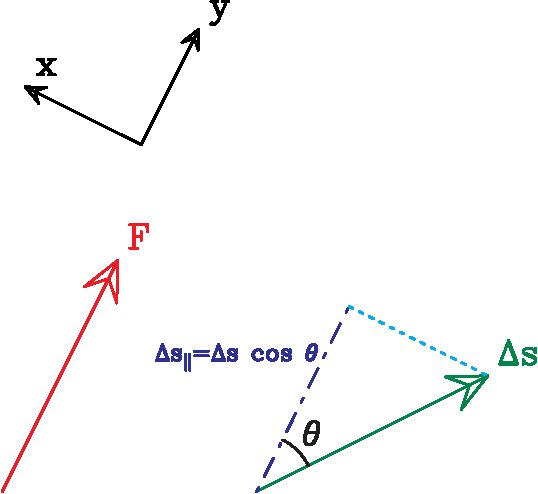
\includegraphics[width=0.6\textwidth]{dp1-crop.pdf}}
		\BI
		\item{$\vec F \cdot \Delta \vec s = (F) (\Delta s_\parallel) = (F) (\Delta s \cos \theta)$}
		\item{``The component of the displacement parallel to the force, times the force}
		\EI
		
		\column{0.5\textwidth}
		\centerline{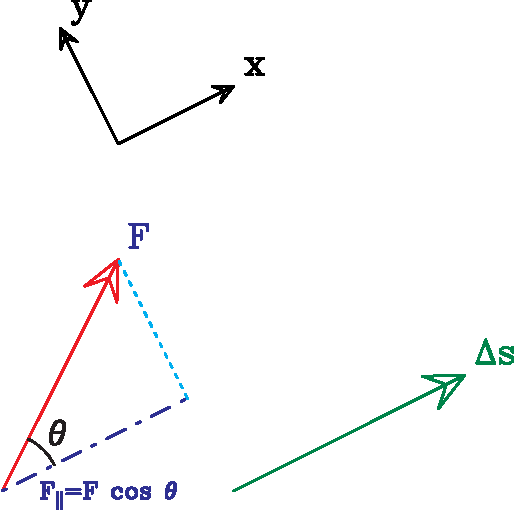
\includegraphics[width=0.6\textwidth]{dp2-crop.pdf}}
		\BI
		\item{$\vec F \cdot \Delta \vec s = (F_\parallel) (\Delta s) = (F \cos \theta) (\Delta s)$}
		\item{``The component of the force parallel to the motion, times the displacement}
		\EI
		
		
	\end{columns}
	\large
	\bigskip
	\centerline{\color{Red}Different cases where each form is useful, but it's the same trig either way}
}




\frame{\frametitle{\textbf{Sample problem: balls on ramps}}
\large
(on document camera)

\pause
\bigskip
\bigskip
\bigskip

Strategy: compute the work done by all the forces and equate that to the change in KE.

\bigskip

Work done by normal force = {\bf zero}!

Work done by gravity = $(F)(\Delta s)_\parallel = mg\Delta y = mg(y_0 - y_f)$

\bigskip
\bigskip

\begin{align*}
  KE_f - KE_i =& W_g \\
  \frac{1}{2} mv_f^2 - 0 =& mg (y_0 - y_f) \\ 
\end{align*}
  
\pause
\bigskip

$\rightarrow v_f = \sqrt{2g(y_0 - y_f)}$

\bigskip
\pause
\bigskip

\centerline{\color{Red}No detailed knowledge of the motion required!}
}



\frame{\frametitle{\textbf{Pendulum demos}}
	\large
	\BI
	\item{What is the work done by the string?}
	\pause
	\item{\color{Red}Zero -- it's always perpendicular to the motion!}
	\item{How high will it swing on the other side?}
	\pause
	\item{Gravity does positive work on the way down and negative work on the way up}
	\item{The kinetic energy can't go below zero}
	\item{The height at each end of the swing must be the same!}
	\item{... and the return height can't be greater than the initial height...}
	\EI
	\pause
	\bigskip
	\bigskip
	
	\normalsize
	\centerline{\color{Blue}(If physics stops working and I go splat, have a nice summer!}
}



\frame{\frametitle{\textbf{Potential energy: an accounting trick}}
  \BI
\item{Notice that the work done by gravity depends {\it only} on the change in height.}
\item{Some other forces are like this as well: the work done depends only on initial and final position}
  \BI
\item{These are called {\it conservative forces}}
\item{Soon we'll see that the elastic force is like this too}
\EI
\item{Separate out gravity and all other forces in the work-energy theorem:}
\begin{align*}
KE_f - KE_i &= W_{\rm grav}+ {\color{Grey}W_{\rm{other}}}\\
\frac{1}{2} mv_f^2 - \frac{1}{2} mv_0^2 &= mg (y_0 - y_f) + {\color{Grey}W_{\rm{other}}}
\end{align*}

\pause
\item{Collect all the ``initial'' things on the left and the ``final'' things on the right:}
  \begin{align*}
    \frac{1}{2} mv_0^2& + mgy_0& + W_{\rm{other}} &=& \frac{1}{2}mv_f^2 &+ mgy_f\\
    KE_0& + GPE_0& + W_{\rm{other}}& =& KE_f &+ GPE_f 
  \end{align*}
\item{Identify $mgy$ as ``gravitational potential energy'': how much work will gravity do if something falls?}
  \EI

\bigskip

\centerline{\color{Red} Potential energy lets us easily calculate the work done by conservative forces}
}

\frame{\frametitle{\textbf{Potential energy: more than accounting!}}
  \BI
\item{Another way to look at the roller coaster: {\color{Red} gravitational potential energy being converted to kinetic energy.}}
\item{This perspective is universal: {\color{Blue}all} forces just convert energy from one sort into another}
\item{Some of these types are beyond the scope of this class, but we should be aware of them!}
\EI
\bigskip
\bigskip
A short history of energy conversion:
\small
\begin{columns}
  \column{0.5\textwidth}  
\BI
\item{Hydrogen in the sun fuses into helium}
\item{Hot gas emits light}
\item{Light shines on the ocean, heating it}
\item{Seawater evaporates and rises, then falls as rain}
\item{Rivers run downhill}
\item{Falling water turns a turbine}
\item{Turbine turns coils of wire in generator}
\item{Electric current ionizes gas}
\item{Recombination of gas ions emits light}
  \EI
  \column{0.5\textwidth}
\BI
\item{Nuclear energy $\rightarrow$ thermal energy}
\item{Thermal energy $\rightarrow$ light}
\item{Light $\rightarrow$ thermal energy}
\item{Thermal energy $\rightarrow$ gravitational potential energy}
\item{Gravitational PE $\rightarrow$ kinetic energy and sound} 
\item{Kinetic energy in water $\rightarrow$ kinetic energy in turbine}
\item{Kinetic energy $\rightarrow$ electric energy}
\item{Electric energy $\rightarrow$ chemical potential energy}
\item{Chemical PE $\rightarrow$ light}
\EI
\end{columns}
}

\frame{\frametitle{\textbf{Potential energy: more than accounting!}}
\BI
\item{This class is just the study of motion: we can't treat light or nuclear energy here.}
\item{... but in physics as a whole, the {\it conservation of energy} -- that processes just change energy from one form to another -- is universal!}
\item{Conservation of energy is one of the most tested, ironclad ideas in science}
\item{Nuclear and chemical potential energy: nuclear forces do mechanical work on particles, much like gravity}
\item{Light, and others: kinetic energy of little particles called ``photons''}
\item{Heat: kinetic energy of atoms in random motion}
\item{Sound: kinetic energy of atoms in coordinated motion}
\item{Food: Just chemical potential energy...}
\item{... so all of these things aren't as far removed from mechanics after all!}
\item{Einstein: ``Mass is just another form of energy''}
\pause
\item{\color{Red}Maybe it's all, ultimately, just kinetic energy! (I believe it is; others will argue!)}
  \EI
}

%
%\frame{
%\Large
%\begin{center}
%Ask a Physicist: how does a nuclear bomb work (and how is it different from a nuclear power plant)?
%\end{center}
%}


\frame{\frametitle{\textbf{A new force: elasticity and Hooke's law}}
To best see how this can be useful, let's introduce a new force: elasticity.

\begin{itemize}

  \item{Springs have a particular length that they like to be: ``equilibrium length'' $L_0$}
  \item{A spring stretched to be longer than this pulls inward to shorten itself}
  \item{A spring compressed to be shorter than this pushes outward to lengthen itself}
  \item{Flexible things like strings and ropes only pull; they kink instead of compressing}
  \item{The force is proportional to the deviation from the optimum length}
\EI
\centerline{    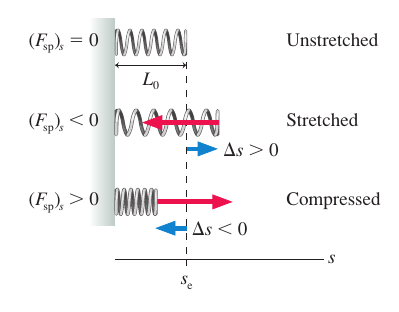
\includegraphics[width=0.4\textwidth]{hooke.png}}
\Large
\centerline{$F_{\rm{elastic}} = -k (L - L_0) = -k \Delta x$ (Hooke's law)}

\bigskip
\pause
\large
$k$ is called the ``spring constant'':

\BI
\item{Measures the stiffness of the spring/rope}
\item{Units of newtons per meter: ``restoring force of $k$ newtons per meter of stretch''}
  \EI
}


\frame{\frametitle{\textbf{A simple spring problem: done with the work-energy theorem}}
\Large
A person of mass $m=100 kg$ falls from a height of $h=3$m onto a trampoline. If the person makes an impression $d=40$ cm deep on the trampoline when he lands, what is the spring constant?

\pause
\bigskip
\bigskip
\bigskip

\normalsize

\BI
\item{Initial kinetic energy + work done by spring + work done by gravity = final kinetic energy}
  \BI
\item{Need to use the integral form of the work-energy theorem since the force isn't constant}
  \EI
\item{The person begins and ends at rest, so we know the initial and final kinetic energy is zero}
\item{The trampoline begins at its equilibrium position}
  \pause
\item{\color{Red}$W_{\rm{grav}} = (mg)(h+d)$}
  \pause
\item{\color{Blue}$W_{\rm{elas}} = \int_0^{-d} \, kx \, dx = -\frac{1}{2} kd^2$}
  \pause
\item{$KE_0 + {\color{Red}W_{\rm{grav}}} + {\color{Blue}W_{\rm{elas}}} = KE_f$}
\item{$0 + \color{Red}(mg)(h+d) \color{Blue}-\frac{1}{2} kd^2 \color{Black}= 0$}
\item{$k = \frac{mg(h+d)}{2d^2}$}
  \EI
}
  

\frame{\frametitle{\textbf{Potential energy stored in a spring}}
\Large 
We saw that an object at height $h$ has gravitational potential energy $mgh$. Can we do something similar for springs?

\large

\bigskip
\bigskip
\pause
\BI
\item{Potential energy, remember, is the work done by some force as it returns to some ``zero'' position.}
\item{A natural choice is $\Delta x=0$, the equilibrium position of the spring.}
  \EI

\Large

``How much work is done by a spring as it goes from $\Delta x=a$ to $\Delta x=0$?

\bigskip
\bigskip

\centerline{$U_{\rm{elastic}} = W_{a \rightarrow 0} = \int_a^0 \, -kx \, dx = \int_0^a \, kx \, dx = \frac{1}{2}ka^2$}

\pause
\bigskip
\bigskip

Now that we have this, we never have to do this integral again!

\bigskip

\centerline{$U_{\rm{elastic}} = \frac{1}{2} kx^2$, where $x$ is the distance from equilibrium}

}


  
  
   
  \frame{\frametitle{\textbf{A simple spring problem: done with potential energy}}
\Large
A person of mass $m=100$ kg falls from a height of $h=3$m onto a trampoline. If the person makes an impression $d=40$ cm deep on the trampoline when he lands, what is the spring constant?

\pause
\bigskip
\bigskip
\bigskip

\normalsize

\BI
\item{Initial total energy + work done by other forces = final total energy}
\item{We have no ``other forces'': we're accounting for gravity and elasticity using potential energy}
\item{The person begins and ends at rest, so we know the initial and final kinetic energy is zero}
\item{Put $y=0$ at the surface of the trampoline}
  \pause
\item{$U_{\rm{grav},0} = mgh$}
\item{$U_{\rm{elas},0} = 0$ (trampoline starts at equilibrium)}
\item{$U_{\rm{grav},f} = -mgd$ (the person falls below $y=0$; PE can be negative!)}
\item{$U_{\rm{elas},f} = \frac{1}{2}kd^2$ (see last slide)}
  \pause
\item{${\color{Lg}KE_0} + U_{\rm{grav},0} + {\color{Lg}U_{\rm{elas},0}} = {\color{Lg}KE_f} + U_{\rm{grav},f} + U_{\rm{elas},f}$}
  \pause
\item{$0 + mgh + 0 = 0 + (-mgd) + \frac{1}{2}kd^2$ (Same terms, maybe on different side)}
  \pause
\item{$k = \frac{mg(h+d)}{2d^2}$}
  \EI
}
  \frame{\frametitle{\textbf{That spring problem: a recap}}
     \large
     \centerline{We don't care about time $\rightarrow$ energy methods}

     \bigskip
     \normalsize

     \begin{columns}
     \column{0.5\textwidth}
     \centerline{Work-energy theorem}
     \column{0.5\textwidth}
     \centerline{Potential energy treatment}
   \end{columns}
   \begin{columns}
     \column{0.5\textwidth}

     \BI
   \item{Initial KE + all work done = final KE}
   \item{Need to compute work done by gravity: easy}
   \item{Need to compute work done by spring: harder\\(need to integrate Hooke's law)}
   \EI
   \column{0.5\textwidth}
   \BI
 \item{Initial KE + initial PE + other work = final KE + final PE}
 \item{No ``other work'' in this problem; all forces have a PE associated}
 \item{Need to know the expressions for PE:}
   \BI
 \item{$U_{\rm{grav}} = mgy$}
 \item{$U_{\rm{elas}} = \frac{1}{2}kx^2$ (x is the distance from the equilibrium point)}
   \EI
 \item{No integrals required (they're baked into the above)}
   \EI
 \end{columns}
 }

 \frame{\frametitle{\textbf{Potential energy with other forces}}
   \large
   What about associating a potential energy with other forces?\normalsize
   \BI
 \item{Friction is a no-go: the work done by friction depends on the path, not just where you start and stop}
 \item{``Ephemeral'' forces like tension and normal force are easiest to deal with by computing work directly}
% \item{The other force we've studied that is easily associated with a potential energy is {\bf universal gravitation}}
%   \BI
% \item{Need to choose a point to set $U=0$; here we choose $r = \infty$}
% \item{$U_G$ = ``work done by gravity on $m_1$ when it moves infinitely far from $m_2$}
%   \EI
\EI
%
%\bigskip
%\bigskip
%
%\Large
%
%   $F_G = \frac{Gm_1 m_2}{r^2}$
%   
%\bigskip
%
%   $W_G = \int_R^\infty\, -\frac{Gm_1m_2}{r^2}\, dr = -\frac{Gm_1 m_2}{R}$
%
%   \pause
%   \bigskip
%
%   $\rightarrow$ Gravitational potential energy between two objects separated by a distance $r$ is $-\frac{Gm_1m_2}{r}$.
 }
%
% \frame{\frametitle{\textbf{The Earth's ``gravity well''}}
%   \large
%    \BI
%  \item{With this choice of the zero point at $r=\infty$, gravitational potential energy is always negative}
%  \item{We have to {\it add energy} to get something away from Earth}
%\EI  
%\bigskip
%
%\centerline{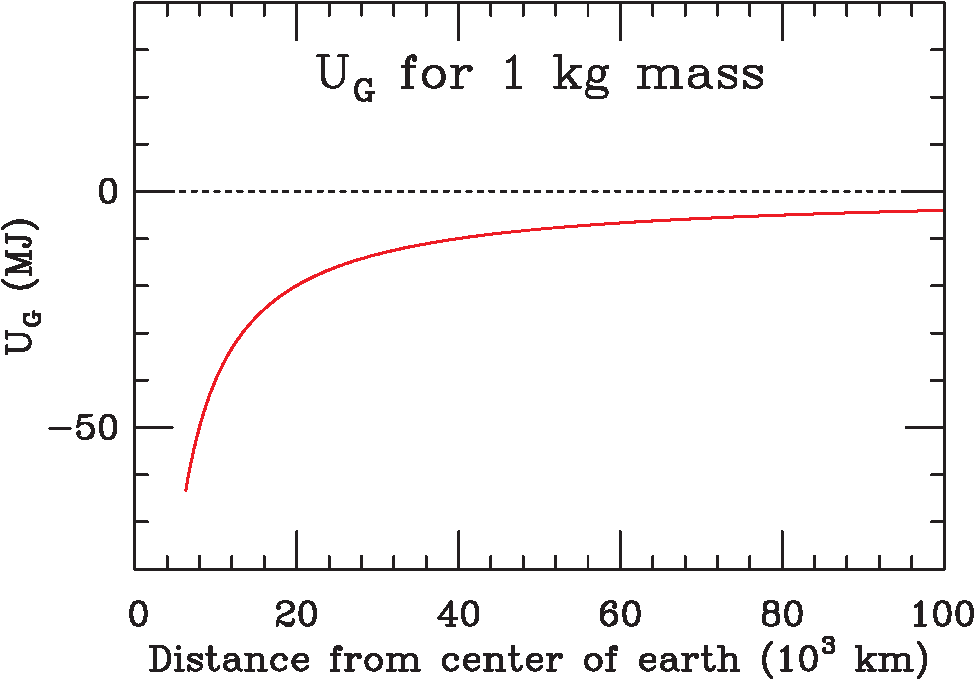
\includegraphics[width=0.6\textwidth]{ug-crop.pdf}}
%
%\bigskip
%
%This region of large negative potential energy is often called a ``gravity well''.
%}

 \frame{\frametitle{\textbf{Summary}}
\large
   \BI
 \item{Potential energy is two things:}
   \BI
 \item{An accounting device that makes it easier to keep track of work done}
 \item{Part of {\it conservation of total energy}, a powerful statement about nature}
   \EI
 \item{Gravitational potential energy (on Earth): $U_g = mgy$}
   \pause
 \item{We learned about a new force: {\bf elasticity}}
   \BI
 \item{Restoring force in a stretched or compressed spring, or a stretched string: }
   \large   \centerline{$F = -k(x-x_0)$ ($x_0$ is the equilibrium length)} \normalsize
 \item{$k$ is the spring constant, measured in force per distance, that gauges stiffness}
 \item{Elastic potential energy: $U_{\rm{elas}}=\frac{1}{2}k(x-x_0)^2$}
   \EI
%\pause
%\item{Gravitational potential energy in general: $U_G = -\frac{Gm_1 m_2}{r}$}
\EI
 }
   \end{document}
